\documentclass[12pt,a4paper]{article}
\usepackage[brazilian]{babel}
\usepackage{amsmath}
\usepackage{amsfonts}
\usepackage{amssymb}
\usepackage[utf8x]{inputenc}
\setlength{\parindent}{1.5em}
\setlength{\parskip}{0.5em}
\usepackage{indentfirst}
\usepackage{float}
\usepackage{systeme}
\usepackage[bitstream-charter]{mathdesign}
\usepackage[T1]{fontenc}
% \usepackage[frenchmath]{newtxmath}
\usepackage[frenchmath]{mathastext}
% \renewcommand*\oldstylenums[1]{{\firaoldstyle #1}}
\usepackage[titles]{tocloft}
\renewcommand{\cftdot}{}
\usepackage[colorlinks=true, allcolors=magenta, backref=page]{hyperref}
\usepackage{url}
\usepackage{graphicx}
%\usepackage{sectsty}
%\allsectionsfont{\mdseries\scshape}

\usepackage{geometry}
 \geometry{
 a4paper, 
 left=2.0cm,
 right=1.6cm,
 top=2.0cm,
 bottom=1.6cm
}

% Colors
\usepackage[dvipsnames]{xcolor}
\newcommand\crule[3][black]{\textcolor{#1}{\rule{#2}{#3}}}
\definecolor{fireopal}{rgb}{0.93, 0.38, 0.33}
\definecolor{aquamarine}{rgb}{0.38, 0.83, 0.58}
\definecolor{mintgreen}{rgb}{0.67, 0.97, 0.51}
\definecolor{crayola}{rgb}{1, 0.85, 0.49}
\definecolor{tangerine}{rgb}{1, 0.61, 0.52}

\usepackage{amsthm}
\newtheoremstyle{break}%
{}{}%
{\itshape}{}%
{\bfseries}{}% % Note that final punctuation is omitted.
{\newline}{}
%\theoremstyle{break}
\theoremstyle{definition}
\newtheorem{theorem}{Teorema}
\newtheorem{corollary}[theorem]{Corolário}
\newtheorem{lemma}[theorem]{Lema}
\newtheorem{remark}[theorem]{Observação}
\newtheorem{proposition}[theorem]{Proposição}
\newtheorem{example}{Exemplo}
\newtheorem{definition}{Definição}
\renewcommand\qedsymbol{$\blacksquare$}

% NEW COMMANDS
\newcommand\restr[2]{{% we make the whole thing an ordinary symbol
  \left.\kern-\nulldelimiterspace % automatically resize the bar with \right
  #1 % the function
  \vphantom{\big|} % pretend it's a little taller at normal size
  \right|_{#2} % this is the delimiter
  }}
  
% TIKZ
\usepackage{pgfplots}
\pgfplotsset{width=7cm,compat=1.8}
\usepackage{pgfplotstable}
% Create a function for generating inverse normally distributed numbers using the Box–Muller transform
\pgfmathdeclarefunction{invgauss}{2}{%
  \pgfmathparse{sqrt(-2*ln(#1))*cos(deg(2*pi*#2))}%
}
\makeatletter
\pgfplotsset{
    table/.cd,
    brownian motion/.style={
        create on use/brown/.style={
            create col/expr accum={
                (\coordindex>0)*(
                    max(
                        min(
                            invgauss(rnd,rnd)*0.1+\pgfmathaccuma,
                            \pgfplots@brownian@max
                        ),
                        \pgfplots@brownian@min
                    )
                ) + (\coordindex<1)*\pgfplots@brownian@start
            }{\pgfplots@brownian@start}
        },
        y=brown, x expr={\coordindex},
        brownian motion/.cd,
        #1,
        /.cd
    },
    brownian motion/.cd,
            min/.store in=\pgfplots@brownian@min,
        min=-inf,
            max/.store in=\pgfplots@brownian@max,
            max=inf,
            start/.store in=\pgfplots@brownian@start,
        start=0
}
\makeatother

% Initialise an empty table with a certain number of rows
\pgfplotstablenew{201}\loadedtable % How many steps?
\pgfplotsset{
        no markers,
        xmin=0,
        enlarge x limits=false,
        scaled y ticks=false,
        ymin=-1, ymax=1
}
\tikzset{line join=bevel} 
  
% FOOTER
\usepackage{fancyhdr}
\pagestyle{fancy}
\fancyhf{}
\fancyhead[LE,RO]{}
\fancyhead[RE,LO]{}
\fancyfoot[LE,LO]{\textbf{XXX Congresso de Iniciação Científica da UNICAMP – 2022}}
\fancyfoot[RE,RO]{\thepage}  
\renewcommand{\headrulewidth}{0pt}
\renewcommand{\footrulewidth}{1pt} 
  
%\usepackage{sectsty}
%\subsectionfont{\color{RubineRed}}
\hypersetup{
    colorlinks=true,
    linkcolor=fireopal,
    filecolor=aquamarine,      
    urlcolor=fireopal,
    pdftitle={An Introduction to Stochastic Differential Equations},
    pdfpagemode=FitH,
}
\author{\href{https://github.com/adairneto}{Adair Antonio da Silva Neto}}
\title{An Introduction to Stochastic Differential Equations}

\begin{document}

%\clearpage\maketitle

\begin{figure}[h]
  \centering
    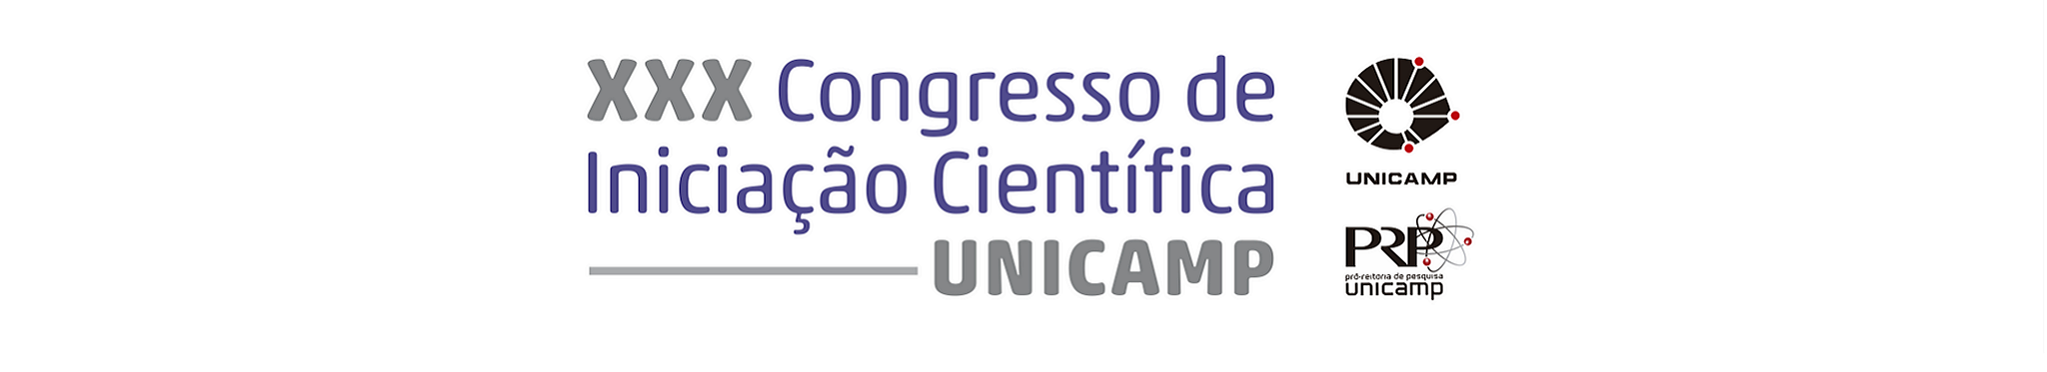
\includegraphics[width=\textwidth]{logo.png}
\end{figure}

\begin{center}
	\LARGE
	\textbf{\uppercase{Introdução às Equações Diferenciais Estocásticas}}
	
	\normalsize
	\textbf{Palavras-chave: Cálculo Estocástico, Movimento Browniano, Ruído Branco}
\end{center}
\begin{flushright}
	\normalsize
	\textbf{Autores: \\
	\uppercase{Adair Antonio da Silva Neto [IMECC - UNICAMP]} \\
	\uppercase{Prof. Dr. Diego Sebastián Ledesma (orientador) [IMECC - UNICAMP]}}
\end{flushright}

\hrule

\section*{Introdução}

Uma equação que modela um processo de evolução que contém ruído, com certa aleatoriedade, seria uma equação da forma:
\begin{equation}\label{eq:sde}
	\frac{\mathrm{d}X}{\mathrm{d}t} = b(t,X_t) + \sigma(t,X_t)\cdot \text{`ruído'}
\end{equation}

Problemas como esse aparecem naturalmente na biologia (modelos de crescimento populacional), física (carga em circuitos elétricos), engenharia (problemas de filtragem como o Filtro de Kalman exibido na Figura \ref{fig:kalman}) e finanças (parada ótima, portfólio ótimo e precificação de opções). 

\begin{figure}[H]
  \centering
    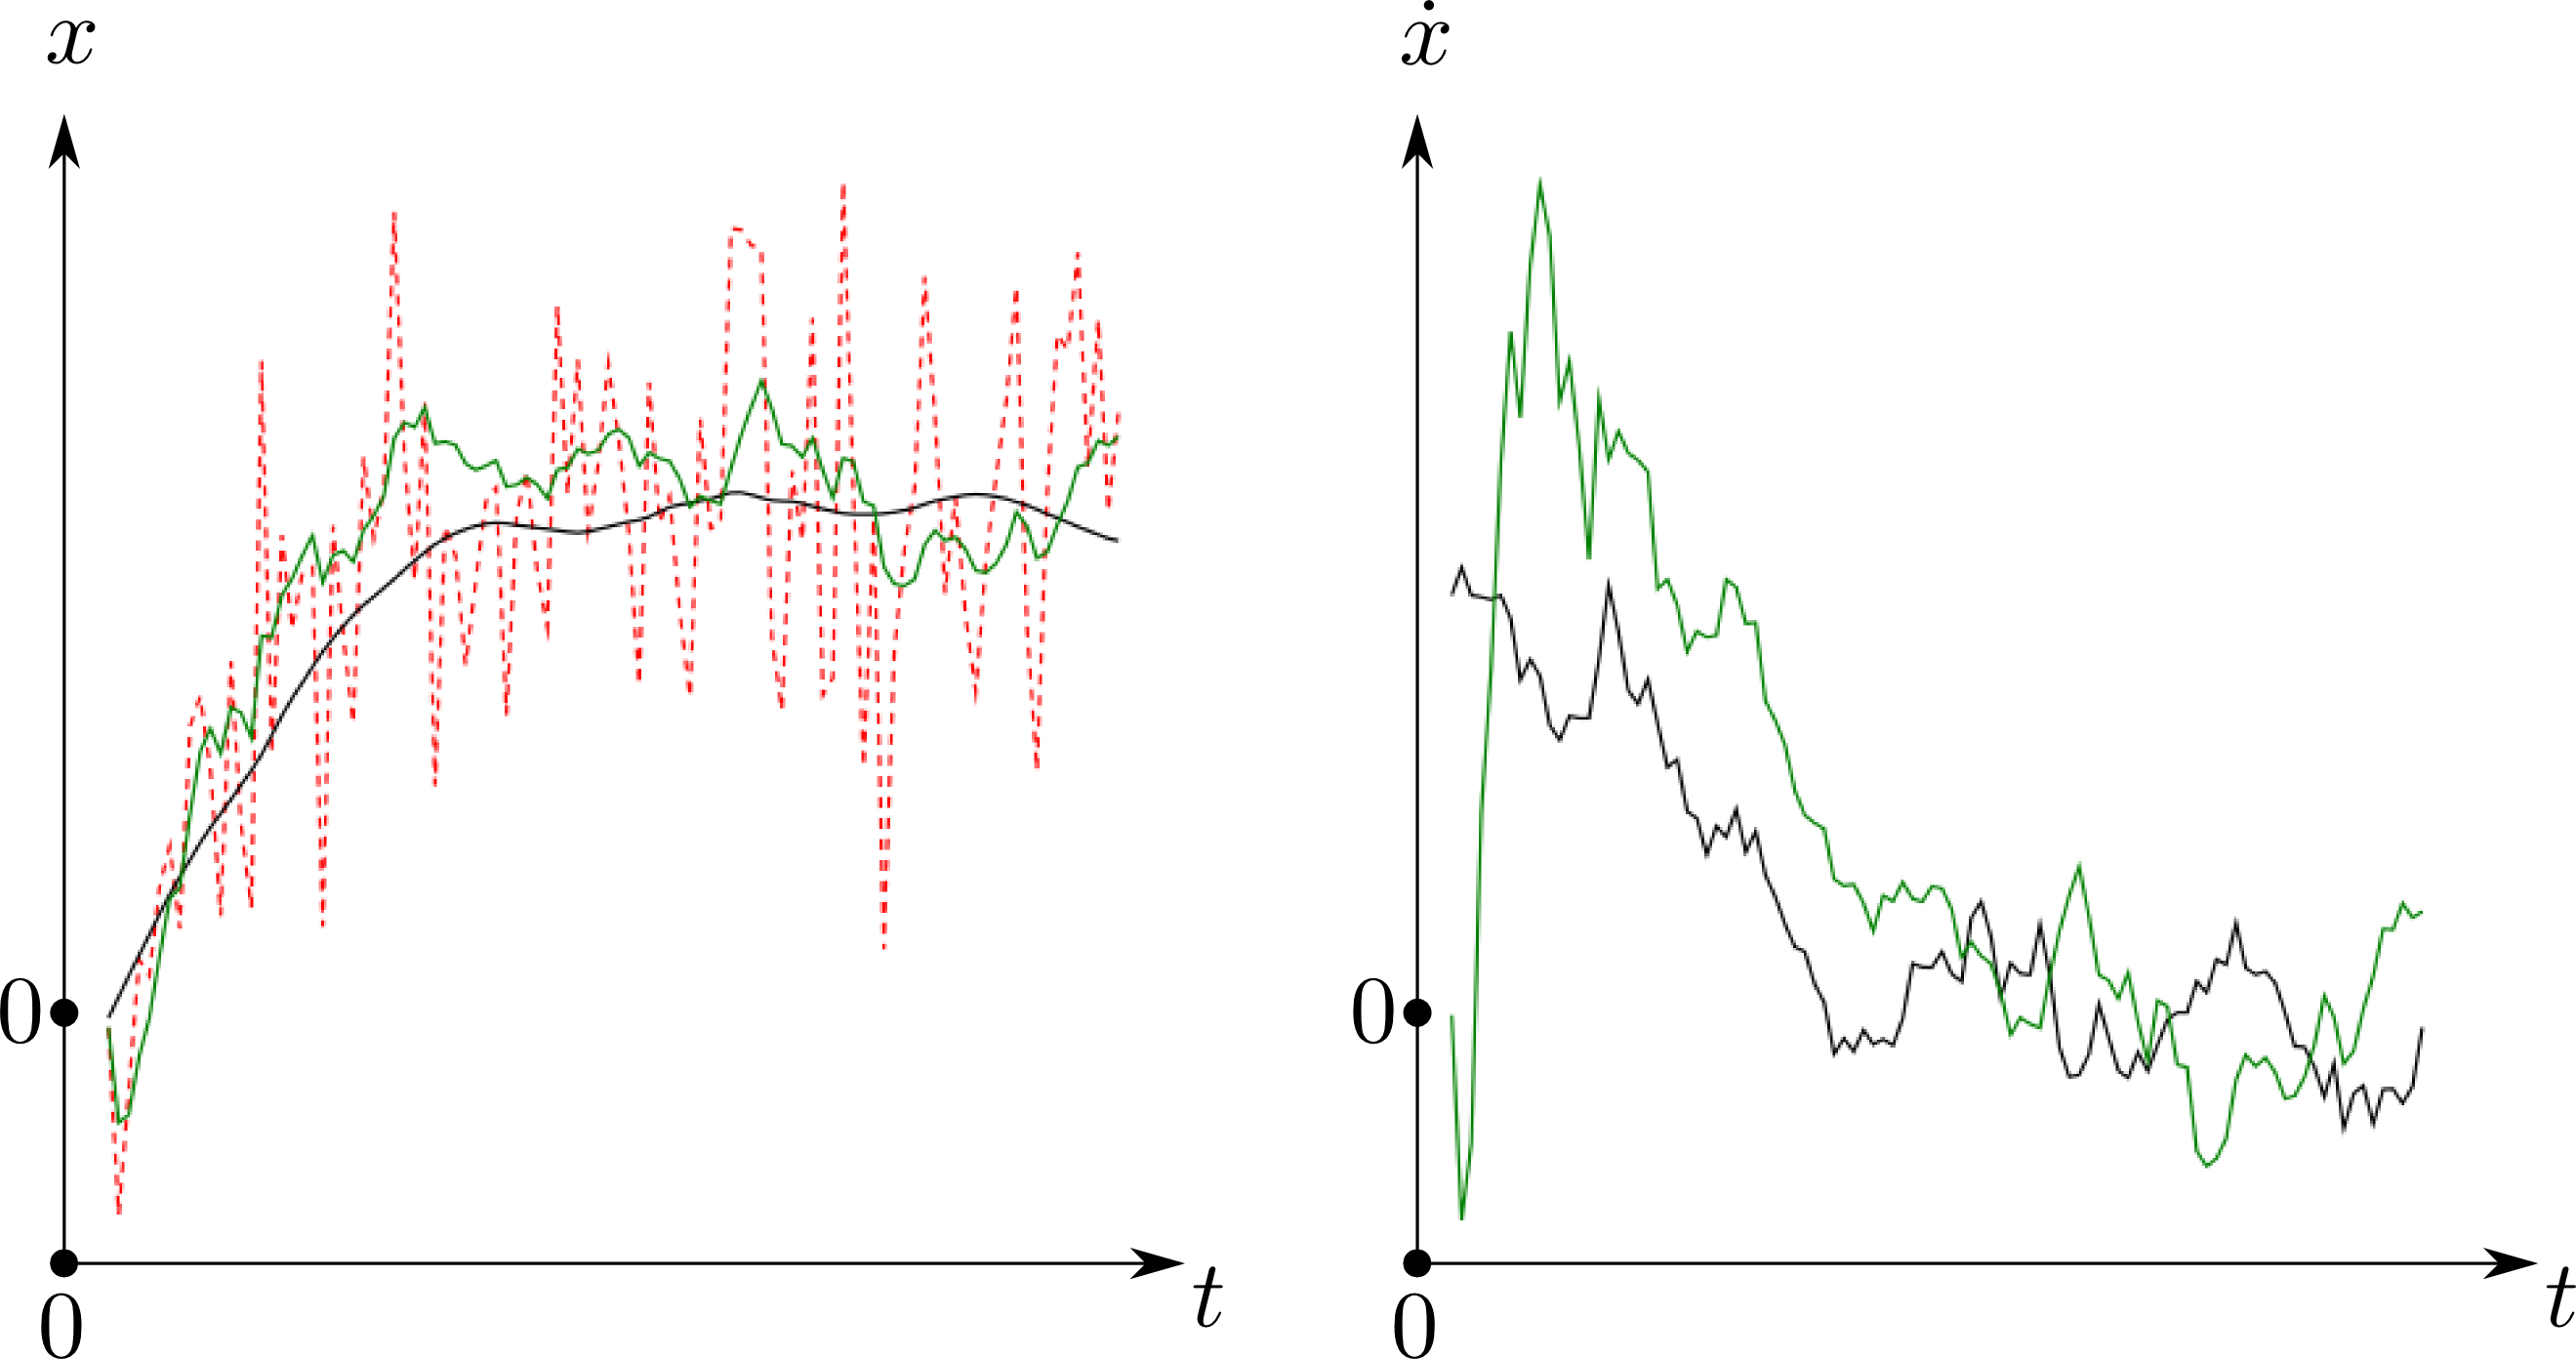
\includegraphics[width=0.7\textwidth]{Kalman.png} 
    \caption{Filtro de Kalman: $\crule[red]{0.4cm}{0.4cm}$ Dados observados; $\crule[ForestGreen]{0.4cm}{0.4cm}$ Processo filtrado; $\crule{0.4cm}{0.4cm}$ Dados reais \cite{wiki:Kalman_filter}.}
    \label{fig:kalman}
\end{figure}

Do ponto de vista matemático, temos que dar sentido a esse tipo de equações, pois com as ferramentas usuais do cálculo diferencial e integral não é possível tratá-las. Nosso objetivo então, neste trabalho, é dar os fundamentos que permitem começar a tratar estas equações. Em particular, definir a integral de Itô.


\section*{Metodologia}

Para estudar a equação \eqref{eq:sde} primeiramente damos uma forma para o `ruído' que vamos considerar. No nosso caso, vamos considerar o `ruído branco', que é um processo estocástico generalizado $W_t$ com distribuição de probabilidade gaussiana de média zero, variância finita tal que $\mathbb{E}[W_sW_t]=0$ sempre que $t\neq s$. No entanto, este processo não tem propriedades razoáveis (não tem caminhos contínuos, não é mensurável para tempo finito). Por causa disso é considerado o movimento Browniano $B_t$ que pode ser visto como um processo estocástico estacionário, com incrementos independentes e média zero tal que 
\[
B_t-B_s=W_s(t-s)
\]
para todo $t\geq s$ isto é, o `ruído branco' é a derivada em relação ao tempo do movimento Browniano. De fato, o único processo que satisfaz essas propriedades é o movimento Browniano (Figura \ref{fig:brownian_motion}). 

\begin{figure}[h!]
\centering
\pgfmathsetseed{3}
\begin{tikzpicture}[scale=1.2]
  \begin{axis}
    \addplot table [
        brownian motion = {%
        	start = 0,	
            max =  0.5,
            min = -0.75
        }
    ] {\loadedtable};
    \addplot table [
        brownian motion = {%
            start =  0,
            min   = -0.5,
            max   =  0.75
        }
    ] {\loadedtable};
  \end{axis}
\end{tikzpicture}
\caption{Simulação de duas realizações do movimento Browniano \cite{texexchange:brownian-tikz}}
\label{fig:brownian_motion}
\end{figure}

Passamos agora ao tratamento da equação. Para isso, observamos que no caso determinístico, em que não há presença de ruído, temos uma equação da forma
\begin{equation}
	\frac{\mathrm{d} X_t}{\mathrm{d} t} = b(t, X_t), \quad X_0 = x_0
\end{equation}

Nesse caso, uma solução é uma função $X_t$ tal que
\begin{equation}
	X_t - X_0 = \int_0^T b(s, X_s) \mathrm{d}s
\end{equation}
Essa função pode ser vista como um processo estocástico sobre um espaço de probabilidade dado por um único ponto. 

Utilizando o formalismo acima propomos como solução à equação \eqref{eq:sde} uma identidade da forma
\begin{equation}\label{eq:sde-sol-prop}
	X_t - X_0 = \int_0^t b(s, X_s) \mathrm{d}s + \int_0^t \sigma(s, X_s) \mathrm{d}B_s
\end{equation}
onde a integral da esquerda é uma integral de Lebesgue-Stieltjes, mas a integral da direita é o que vamos formalizar neste trabalho. 

\section*{Resultados e Discussão}

Como vimos na seção anterior queremos dar sentido à seguinte integral
\begin{equation}\label{eq:gen_ito_integrand}
	\int_S^T f(t, \omega) \mathrm{d}B_t(\omega)
\end{equation}
onde $f : [0, \infty] \times \Omega \longrightarrow \textbf{R}$.

A ideia será a seguinte: começaremos definindo a integral para as funções mais simples possíveis e depois, por aproximações e critérios de convergência, iremos defini-la para as outras classes de funções. Em particular queremos definir a integral para   a classe de funções  $\mathfrak{V}(S,T)$ que está formada por 
	\[
		f(t, \omega) : [0, \infty) \times \Omega \longrightarrow \textbf{R}
	\]
	tais que
	\begin{enumerate}
		\item A função $(t, \omega) \longrightarrow f(t, \omega)$ é $\mathfrak{B} \times \mathfrak{F}$-mensurável, onde $\mathfrak{B}$ denota a $\sigma$-álgebra de Borel em $[0, \infty)$ e $\mathfrak{F}$ é a $\sigma$-álgebra gerada pelas variáveis aleatórias $B_s$ ($s \leq t$).
		\item A função $f(t,\omega)$ é $\mathfrak{F}_t$-adaptada.
		\item $\mathbb{E} \left[ \int_S^T f(t, \omega)^2 \mathrm{d}t \right] < \infty$.
	\end{enumerate}

Começamos então com as funções mais simples. 
\begin{definition}[Funções elementares]
		Uma função $\varphi \in \mathfrak{V}(S,T)$ é dita \textbf{elementar} se é da forma
	\begin{equation}
		\varphi(t, \omega) = \sum_j e_j(\omega) \chi_{[t_j, t_{j+1}]}(t)
	\end{equation}
\end{definition}

Para as funções elementares definimos 
\[
\int_S^T\varphi(t, \omega)~dB_t=\sum_{j}e_j(\omega)(B_{t_{j+1}}(\omega)-B_{t_j}(\omega)).
\]
As funções elementares são importantes porque são densas em $\mathfrak{V}(S,T)$ como garante o seguinte resultado.
\begin{theorem}
Se $g\in \mathfrak{V}(S,T)$  então existe uma sequência de funções elementares $\varphi_n\in \mathfrak{V}(S,T)$ tal que $\varphi_n\to g$ em $L^2(P)$
\end{theorem}

E, a partir disso, podemos definir a integral \eqref{eq:gen_ito_integrand} com a seguinte definição.

\begin{definition}[Integral de Itô]
	Seja $f \in \mathfrak{V}(S,T)$, então a \textbf{Integral de Itô} de $f$, de $S$ a $T$ é
	\begin{equation}
		\int_S^T f(t, \omega) \mathrm{d}B_t(\omega) = \lim_{n \to \infty} \int_S^T \varphi_n (t, \omega)  \mathrm{d}B_t(\omega)
	\end{equation}
	onde o limite é em $L^2(P)$ e $( \varphi_n )$ é uma sequência de funções elementares tais que
	\[
		\mathbb{E} \left[ \int_S^T (f(t, \omega) - \varphi_n(t, \omega))^2 \mathrm{d}t \right] \longrightarrow 0
	\] 
	quando $n \to \infty$.
\end{definition}

Com a integral de Itô já bem definida, enunciaremos a Isometria de Itô e um corolário, listaremos algumas propriedades e, por fim, daremos um exemplo do cálculo dessa integral.

\begin{theorem}[Isometria de Itô]
	Para toda função $f \in \mathfrak{V}(S,T)$,	
	\begin{equation}
		\mathbb{E}\left[\left( \int_S^T f(t,\omega) \mathrm{d}B_t(\omega) \right)^2 \right] = \mathbb{E} \left[\int_S^T f(t,\omega)^2 \mathrm{d}t \right]
	\end{equation}
\end{theorem}

\begin{corollary}\label{cr:ito}
	Se $f(t, \omega) \in \mathfrak{V}(S,T)$, $f_n(t, \omega) \in \mathfrak{V}(S,T)$ e
	\[
		\mathbb{E}\left[\left( \int_S^T f_n(t,\omega) - f(t, \omega) \right)^2 \mathrm{d}t \right] \longrightarrow 0
		\]
	quando $n \to \infty$, então
	\begin{equation}
		\int_S^T f_n(t, \omega) \mathrm{d}B_t(\omega) \longrightarrow \int_S^T f(t, \omega) \mathrm{d} B)t(\omega)
	\end{equation}
	em $L^2(P)$ conforme $n \to \infty$.
\end{corollary}

De fato, a integral de Itô possui as propriedades esperadas de uma integral e, além disso, tem média zero e é $\mathfrak{F}_T$-mensurável.

\begin{theorem}[Propriedades]
	Seja $f, g \in \mathfrak{V}(0,T)$ e $0 \leq S < U < T$. Então
	\begin{enumerate}
		\item $\int_S^T f \mathrm{d}B_t = \int_S^U f \mathrm{d}B_t + \int_U^T f \mathrm{d}B_t$ para $\omega$ em quase toda parte.
		\item $\int_S^T (cf + g) \mathrm{d}B_t = c \int_S^T f \mathrm{d}B_t + \int_S^T g \mathrm{d}B_t$ onde $c \in \textbf{R}$.
		\item $\mathbb{E} \left[ \int_S^T f \mathrm{d}B_t \right] = 0$.
		\item $\int_S^T f \mathrm{d}B_t$ é $\mathfrak{F}_T$-mensurável.
	\end{enumerate}
\end{theorem}

\begin{example}
	Queremos calcular a integral
	\[
		\int_0^T B(t) \mathrm{d}B(t)
	\]
		
	\textbf{Passo 1.} Seja
	\[
		\varphi_n(t) = \sum_{i=0}^{n-1} B_n(t_i^n)[B_n(t_{i+1}^n) - B_n(t_i^n)]
	\]
	uma sequência de funções elementares. Então,
	\begin{equation*}
		\begin{aligned}
			\mathbb{E} \left[ \int_0^T (\varphi_n - B_s)^2 \mathrm{d}s \right]
			&= \mathbb{E} \left[ \sum_j \int_{t_j}^{t_{j+1}} (B_j - B_s)^2 \mathrm{d}s \right]
			= \sum_j \int_{t_j}^{t_{j+1}} (s - t_j)^2 \mathrm{d}s \\
			&= \sum_j \frac{1}{2} \left(t_{j+1} - t_j \right)^2 \longrightarrow 0 \, \text{ quando } \Delta t_j \to 0
		\end{aligned}
	\end{equation*}
	
	Isto é, pela continuidade de $B(t)$, $\varphi_n(t)$ converge para $B(t)$ quase certamente quando $\Delta t_j \to 0$.
	
	\textbf{Passo 2.} Agora note que
	\begin{equation*}
		\begin{aligned}
			B_n(t_i)[B_n(t_{i+1}) - B_n(t_i)] &= B_n(t_{i+1}) B_n(t_i) - B_n^2(t_i) + B_n^2(t_{i+1}) - B_n^2(t_{i+1}) \\
			&= \frac{1}{2} [B_n^2(t_{i+1}) - B_n^2(t_i) - (B_n(t_{i+1}) - B_n(t_i))^2 ]
		\end{aligned}
	\end{equation*}
	
	\textbf{Passo 3.} Com esses dois resultados e o corolário \eqref{cr:ito}, podemos reescrever a integral original como
	\[
		\int_0^T \varphi_n(t) \mathrm{d}B(t) = \frac{1}{2} \sum_{i=0}^{n-1} \left[ B_n^2(t_{i+1}) - B_n^2(t_i) \right] - \frac{1}{2} \sum_{i=0}^{n-1} \left[ B_n(t_{i+1}) - B_n(t_i) \right]^2
	\]
	
	\textbf{Passo 4.} Como a primeira soma é uma soma telescópica e a segunda soma converge em probabilidade para $T$ pela variação quadrática do movimento Browniano, temos que
	\[
		\int_0^T \varphi_n(t) \mathrm{d}B(t) = \frac{1}{2} B^2(t) - \frac{1}{2} B^2(0) - \frac{1}{2}T = \frac{1}{2} B^2(t) - \frac{1}{2}T 
	\]
	
	Logo, a integral converge em $L^2(P)$ para
	\begin{equation}
		\int_0^T B(t) \mathrm{d}B(t) = \lim_{n \to \infty} \int_0^T \varphi_n(t) \mathrm{d}B(t) = \frac{1}{2} B^2(t) - \frac{1}{2}T 
	\end{equation}
\end{example}

% O próximo resultado afirma que a integral de Itô é um martingale e apresenta uma importante desigualdade.

% Mas antes disso, o que é um martingale? 

% \begin{definition}[Martingale]
% 	Um processo estocástico $\{M_t \}$ on $(\Omega, \mathfrak{F}, P)$ é chamado de \textbf{martingale} com respeito à filtração $\mathfrak{M}_t$ se 
% 	\begin{enumerate}
% 		\item $M_t$ é $\mathfrak{M}_t$-mensurável para todo $t$.
% 		\item $\mathbb{E}[|M_t|] < \infty$ para todo $t$.
% 		\item $\mathbb{E}[M_s | \mathfrak{M}_t] = M_t$ para todo $s \geq t$.
% 	\end{enumerate}
% \end{definition}

% Intuitivamente, um martingale é um processo estocástico no qual o valor esperado de qualquer ponto no futuro é igual ao valor esperado do processo no momento presente.

\section*{Conclusões}

Apresentamos um formalismo para a modelagem de processos de evolução com ruído a partir do movimento Browniano. Vimos que o conceito de solução clássico não funciona para esse formalismo e foi proposta uma nova interpretação. Como resultado disso, foi necessário construir uma nova teoria de integração e, com isso, a integral de Itô. Estudamos as propriedades dessa nova integral. 

A partir disso será possível avançar em questões mais elaboradas, como por exemplo: A equação \eqref{eq:sde} tem solução? Sob quais hipóteses? Como podemos estudar o comportamento da solução?

\nocite{*}
\bibliographystyle{alpha}
\bibliography{XXX_Congresso.bib}

\end{document}